\documentclass[10pt]{article}
\usepackage[margin=1in]{geometry}

\usepackage{amsmath}
\usepackage{amssymb}
\usepackage{graphicx}
\usepackage{url} % for \url{}
%\usepackage[colorlinks = true, urlcolor = {blue}]{hyperref}
%\usepackage[T1]{fontenc}
\usepackage{listings}
\usepackage{color} % for \color{}
\usepackage{threeparttable} % for adding notes beneath table

\title{Connecting multiple sensors over I2C in embedded Linux: \\
an example using a LIDAR-Lite and PX4Flow}

\author{Trevor Avant}
\date{}

\begin{document}

\maketitle
\thispagestyle{empty}
\pagestyle{empty}


%%%%%%%%%%%%%%%%%%%%%%%%%%%%%%%%%%%%%%%%%%%%%%%%%%%%%%%%%%%%%%%%%%%%%%%%%%%%%%%%
\begin{abstract}
This document describes the process of connecting two sensors, a LIDAR-Lite and a PX4Flow optic flow sensor, together over I2C to a Gumstix embedded computer.
\end{abstract}

\section*{Hardware}
\begin{figure}[ht]
\centering
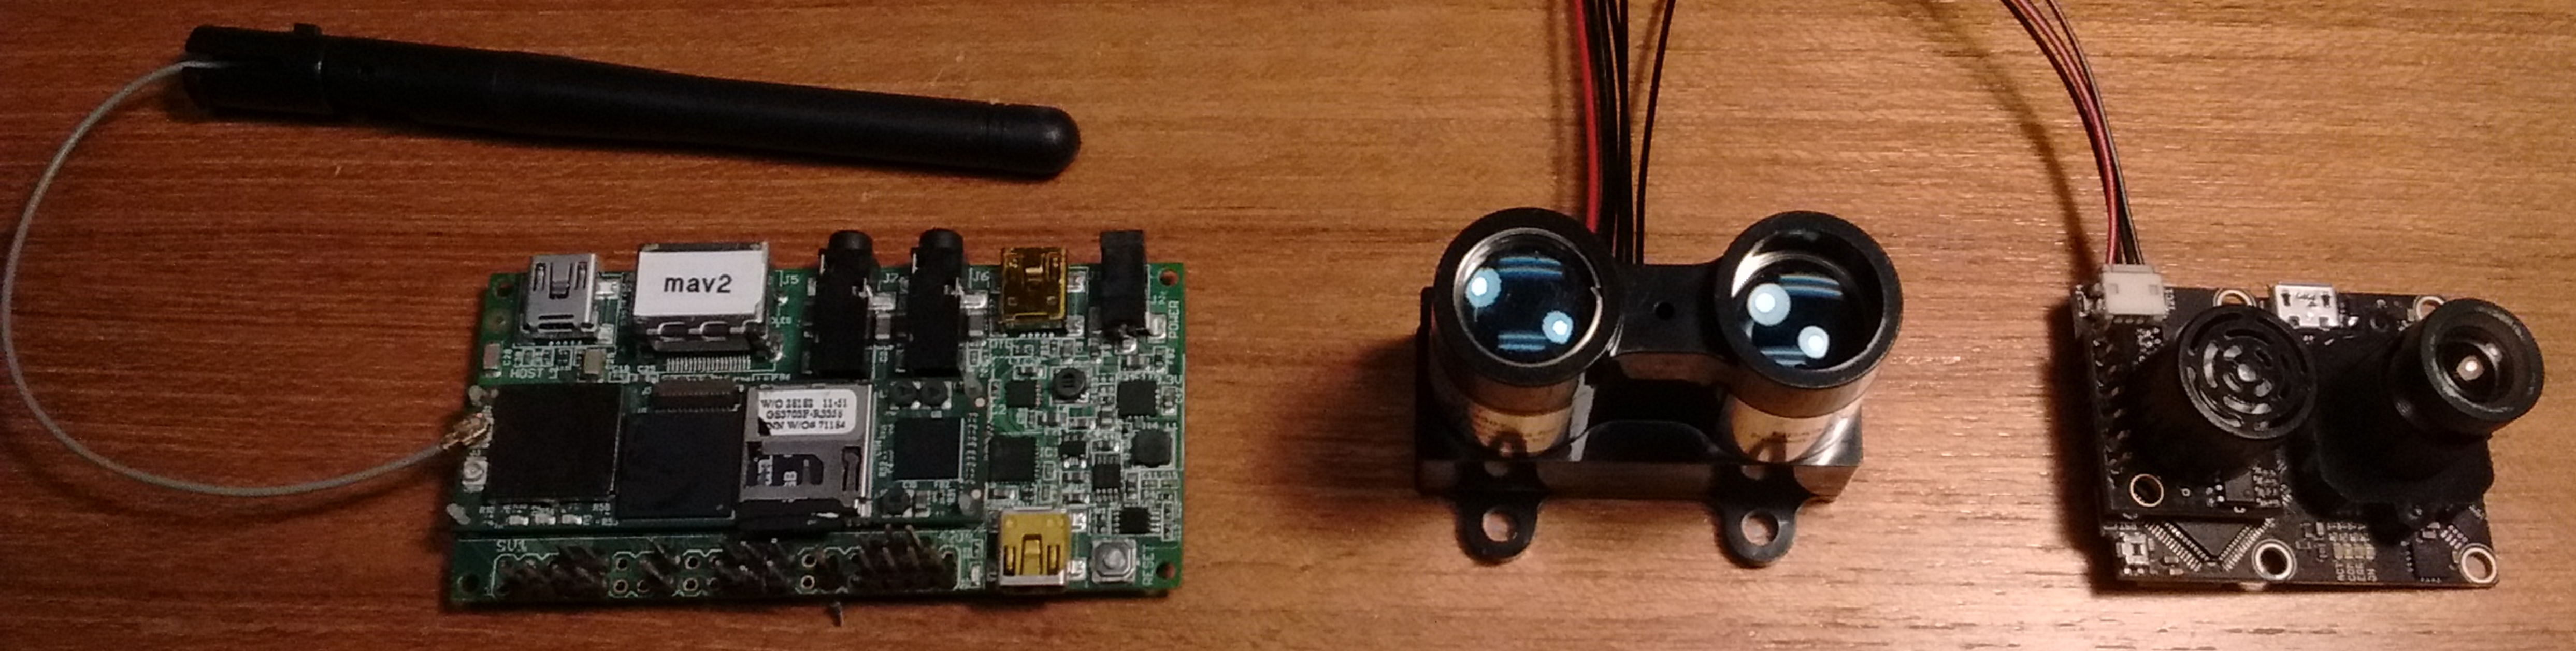
\includegraphics[width=1.0\textwidth]{photos/hardware.pdf}
\caption{Hardware used in the project. Left to right: Gumstix with expansion board, LIDAR-Lite (version 1), PX4Flow (version 1.3).}
\end{figure}
We used a Gumstix Overo FireSTORM COM embedded computer which runs a Linux operating system. We connected this device to a Gumstix SUMMIT expansion board to easily access the I2C output and other outputs. More specifically, the Overo's i2c-3 bus can be accessed via the 40 pin header on the expansion board. The goal of the project was to connect two sensors to the embedded computer over I2C: a LIDAR-Lite (version 1) and a PX4Flow optic flow sensor (version 1.3).

One of the main challenges of interfacing the sensors with the embedded computer is that the i2c-3 bus on the Overo uses 1.8V logic (meaning a binary 1 is represented as 1.8V and a binary 0 is represented as 0V). However, the LIDAR-Lite and PX4Flow both use a 5V logic I2C. Accordingly, it is necessary to use a logic level shifting circuit to convert the 1.8V logic on the Overo to the 5V logic on the sensors.

\section*{I2C in Embedded Linux}
In Overo's Linux environment, we wrote all code to do the I2C communication in user space in the C language. In Linux, communication over I2C can be accomplished by using the \texttt{ioctl} function, which can be included in a C file by the command \texttt{\#include <sys/ioctl.h>}.

Using \texttt{ioctl} to perform I2C operations in user space is not obvious. We have found that a good way to learn how is by examining the i2c-tools package. The i2c-tools source code can be downloaded using \texttt{sudo apt-get source i2c-tools}.
%Note that there is an i2c-tools page on GitHub, but do not use it as some of these files are erroneous.
A particularly useful file in the source code is /include/linux/i2c-dev.h, which shows how to use I2C commands with SMBus functionality. The i2c-tools package can be downloaded and installed, but we chose to use just copy the declarations and definitions we needed from /include/linux/i2c-dev.h. Doing it this way makes it a little more transparent as to how \texttt{ioctl} is being used. For information about the C code we used, see the Appendix.

\section*{LIDAR-Lite and PX4Flow over I2C}
In all I2C communications, the master (in this case the Overo) must specify whether the command sent to the slave (in this case the LIDAR-Lite or PX4Flow) is a ``read'' or ``write'' operation. The format of these read and write operations are dictated by the slave device, and can be determined from the slave device's documentation.

In order to obtain sensor data from the PX4Flow, the master must send a write command specifying what information is to be obtained, and then send a read command in which the master reads the appropriate data. There can be no stop bit between the write and read commands (for definition of a ``stop bit'' in I2C protocol, consult a reference on I2C communication). This write/read sequence can be accomplished using the \texttt{I2C\_RDWR} protocol of the ioctl function (i.e. a command of the form \texttt{ioctl(file, I2C\_RDWR, struct i2c\_rdwr\_ioctl\_data *msgset)}). This function is designed to send combined commands consisting of read and write operations to a device, with no stop bits in between. Note that the \texttt{I2C\_SMBUS} protocol of \texttt{ioctl} (i.e. commands of the form \texttt{ioctl(file, I2C\_SMBUS, struct i2c\_smbus\_ioctl\_data *args)}) cannot be used as we do not believe this function can implement combined read/write sequences with no stop bits in between. Also note that the PX4Flow does not require read and write operations to be sent to specific registers on the device.

To obtain sensor data from the LIDAR-Lite over I2C, the master must send a write command, wait some amount of time for the sensor to do some processing, and then send a read command to finally obtain the data. This requires separate write and read commands to be sent to the LIDAR-Lite (unlike the combined write/read operation for the PX4Flow). The \texttt{I2C\_SMBUS} protocol of the \texttt{ioctl} function can be used to obtain this data. As noted in the \texttt{ioctl} function's documentation, the \texttt{I2C\_SMBUS} protocols are ``not meant to be called directly'', and instead should be called with the help of an access function. 


\section*{Logic Level Shifting Circuit}
As previously noted, the Overo has 1.8V logic while the LIDAR-Lite and PX4Flow use 5V logic. I2C communication between a master and slave with the same logic voltages simply requires the use of two pull-up resistors: one from the supply voltage to the clock line, and one from the supply voltage to the data line. When the master and slave operate at different logic levels, as in this case, a more complicated circuit is required to ensure the logic signals match.

There are a variety of circuits which can perform logic level shifting. We used the circuit described in application note AN10441 provided by NXP (the company which originally created I2C). This circuit uses MOS-FETs in combination with four pull-up resistors. Choosing values for pull-up resistors depends on properties of master and slave devices such as the bus capacitance and the values of internal pull-up resistors on either the master or slave (if such internal pull-ups exist or are enabled). The basic limiting factors for pull-up resistors is as follows.
\begin{itemize}
\item \textit{pull-up resistance too low}: the clock and data lines cannot obtain a low enough voltage to register as a logic 0
\item \textit{pull-up resistance too high}: the clock and data lines will not be able to return to a high state (logic 1) from a low state (logic 0) fast enough before the next clock cycle begins
\end{itemize}

It is possible to calculate appropriate values for pull-up resistors based on characteristics of the circuit (e.g. internal pull-up resistance, bus capacitance, etc.). However, depending on the circuit you are working with, this may be a challenge if the circuit is complex or has unknown characteristics (e.g. a manufacturer does not specify if a sensor has internal pull-up resistors). Instead of calculating pull-up values directly, we used a trial and error method by building a logic level shifting circuit with pull-up resistors of variable resistance. Thus, we built the circuit in application note AN10441, and used potentiometers wired as variable resistors for the pull-up resistors (those labeled as $R_p$ in NXP's diagram). This circuit is shown in Fig. \ref{fig:logic_level_shifing_circuit}.
\begin{figure}[ht]
\centering

\includegraphics[width=1.0\textwidth]{photos/board.pdf}
\caption{Logic level shifting circuit in NXP's application note AN10441, with variable resistors (blue components) used as the pull-up resistors $R_p$. The MOS-FETs are the small, black, rectangular components. CLK denotes the I2C clock line, DAT denotes the I2C data line, and ``sensors'' denotes the LIDAR-Lite and PX4Flow.}
\label{fig:logic_level_shifing_circuit}
\end{figure}
Note that Adafruit makes a breakout board which replicates the AN10441 circuit with 10k resistors (\url{https://www.adafruit.com/product/757}). However, as will be shown in the next section, fixed 10k resistors will not work for all sensor configurations in this project.


\section*{Experimental Investigation of the Circuit}

\subsection*{Working Pull-Up Resistances}

Using the aforementioned circuit with variable resistors, it is easy to test the range of working pull-up resistors for different sensor combinations. Note that all tests in this section were performed at an I2C clock speed of 400 kbit/sec. Table \ref{table:pullup} shows the working ranges for different sensor configurations.
\begin{table}[ht]
\centering
\begin{threeparttable}
\begin{tabular}{| c | c | c | c |} 
\hline
\textbf{Device Tested} & \textbf{Devices Connected} & \textbf{Minimum Pull-Up ($\Omega$)} & \textbf{Maximum Pull-Up ($\Omega$)} \\
\hline
LL & LL & 1k & $\infty$ \\ % lower: more precisely .9k
\hline
PX & PX & 5k & 18k \\ % lower: more precisely 4.5k, upper: formerly 28k $\leq R_p <$ 75k
\hline
LL & LL \& PX & 1k & $\infty$ \\
\hline
PX & LL \& PX & 12k & $\infty$ \\ % upper: formerly 12k?
\hline
\end{tabular}
\begin{tablenotes}
\small
\item *``LL'' denotes LIDAR-Lite and ``PX'' denotes PX4Flow
\end{tablenotes}
\caption{ Minimum and maximum pull-up resistor values $R_p$ for working operation of I2C devices using the level shifting circuit in NXP's AN10441 application note. A value of $\infty$ denotes that the pull-up resistors have been removed entirely from the circuit (i.e. an open circuit).}
\label{table:pullup}
\end{threeparttable}
\end{table}
Interestingly, any sensor configuration in which the LIDAR-Lite is connected will work even if there is an infinite pull-up resistance, i.e. all four pull-up resistors are removed from the circuit entirely! Although this may seem perplexing at first, the 1.8V side of the clock and data lines is still connected to the 5V side through the MOS-FETs. We believe the circuit still works due to internal pull-up resistors on the computer and/or sensors. As a next step, we will gather more insight into the inner workings of the I2C circuit by probing it with an oscilloscope. 

\subsection*{LIDAR-Lite}

Fig. \ref{fig:LL} shows the clock and data lines when only the LIDAR-Lite is connected by itself.
\begin{figure}[ht]
\newcommand{\wdt}{.24\textwidth}
\centering
\iffalse
\includegraphics[width=\wdt]{photos/test.pdf}
\includegraphics[width=\wdt]{photos/test.pdf}
\includegraphics[width=\wdt]{photos/test.eps}
\includegraphics[width=\wdt]{photos/test.pdf}
\includegraphics[width=1.0\textwidth]{photos/LL_withLLonly.pdf}
\caption{I2C waveform (lower: clock line, upper: data line) when the LIDAR-Lite is connected by itself. Checkmarks denote whether the I2C transmission was successful with the corresponding value of pull-up resistor. Note that the small ``$1 \blacktriangleright$'' and ``$2 \blacktriangleright$'' symbols on the far left side indicate 0V for the clock and data lines, respectively.}
\fi
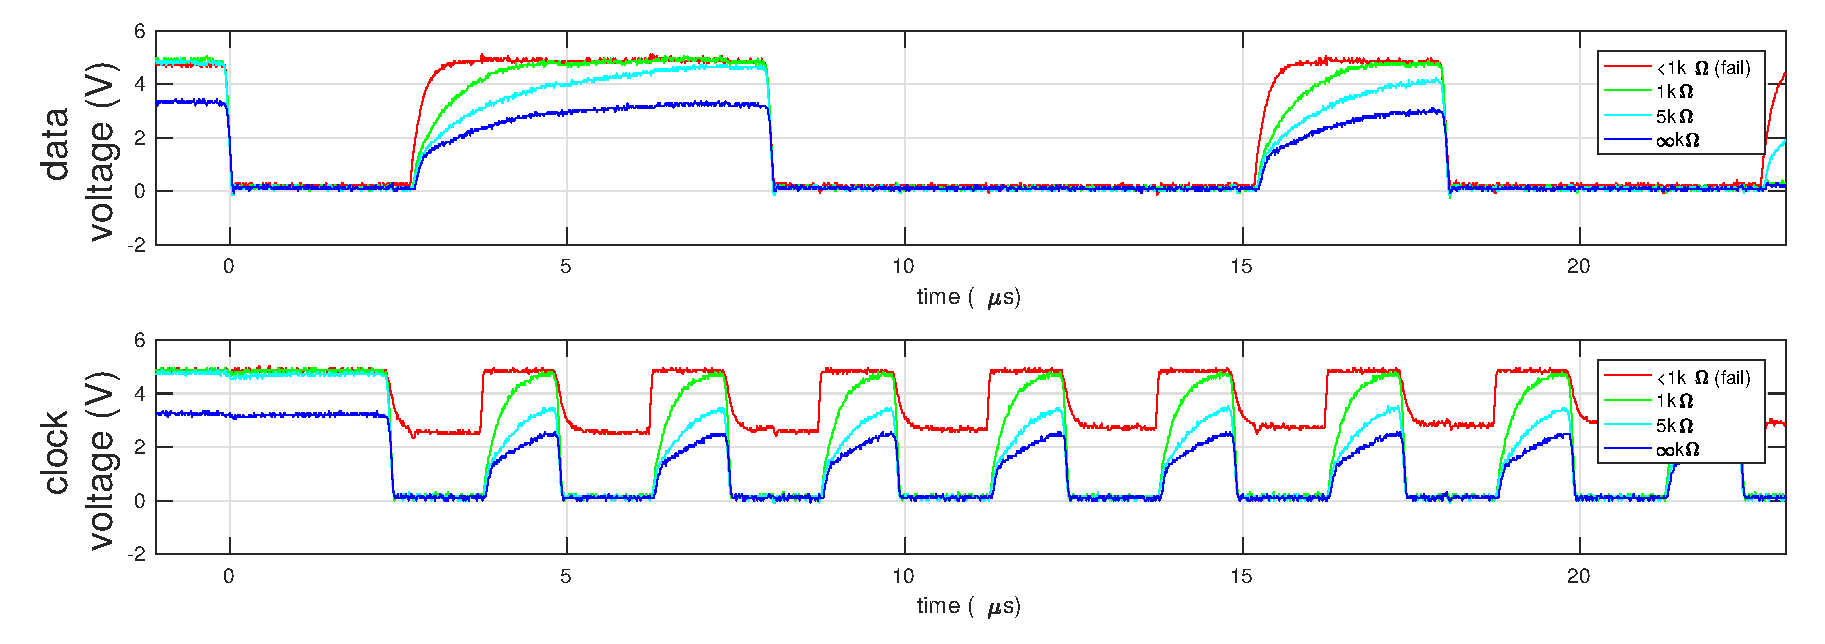
\includegraphics[width=1.0\textwidth]{2pt5microsec/LL_cropped.eps}
\caption{I2C waveform for various pull-up resistors when the LIDAR-Lite is connected by itself. Note that the bits of data transfer can be deduced by comparing the clock cycles to the data line. This sequence is 1100010...}
\label{fig:LL}
\end{figure}
First, let's consider the clock lines. There are two main trends to compare in the different plots. The first is how close to low (0V) the waveform gets. With the $<1k\Omega$ pull-ups, the voltage only gets down to about 2.5V, which is why the I2C communication fails. For the rest of the pull-up values, the clock line gets very close to 0V. The other trend is how fast the waveform reaches high (5V). It is clear that as the pull-up resistance is increased, the clock line is slower to rise to 5V. And actually, with $5 k \Omega$ and $\infty k \Omega$ pull-ups, the clock line is so slow to rise it can't even reach 5V in one clock cycle.  Interestingly, despite the imperfect waveforms of the $5 k \Omega$ and $\infty k \Omega$ plots, the I2C communications still work. Additionally, note that the beginning of the waveform for the $\infty k \Omega$ pull-ups show that the high voltage has actually dropped to about 3V.

Now let's consider the data line in the plots of Fig. \ref{fig:LL}. The data line shows similar trends to the clock line. As the pull-up resistors are increased, the waveform is slower to rise to 5V. For the $\infty k \Omega$ resistance, the voltage only reaches about 3V. However, unlike the clock line, the data line always maintains a low voltage close to 0V.

\subsection*{PX4Flow}

Let's also look at the clock and data waveforms when the PX4Flow is connected by itself. The waveforms are shown in Fig. \ref{fig:PX}.
\begin{figure}[ht]
\centering
\iffalse
\includegraphics[width=1.0\textwidth]{photos/tester.pdf}
\caption{I2C waveform (lower: clock line, upper: data line) when the PX4Flow is connected by itself. Checkmarks denote whether the I2C transmission was successful with the corresponding value of pull-up resistor. Note that the ``$1 \blacktriangleright$'' and ``$2 \blacktriangleright$'' symbols on the far left side indicate 0V for the clock and data lines, respectively.}
\fi
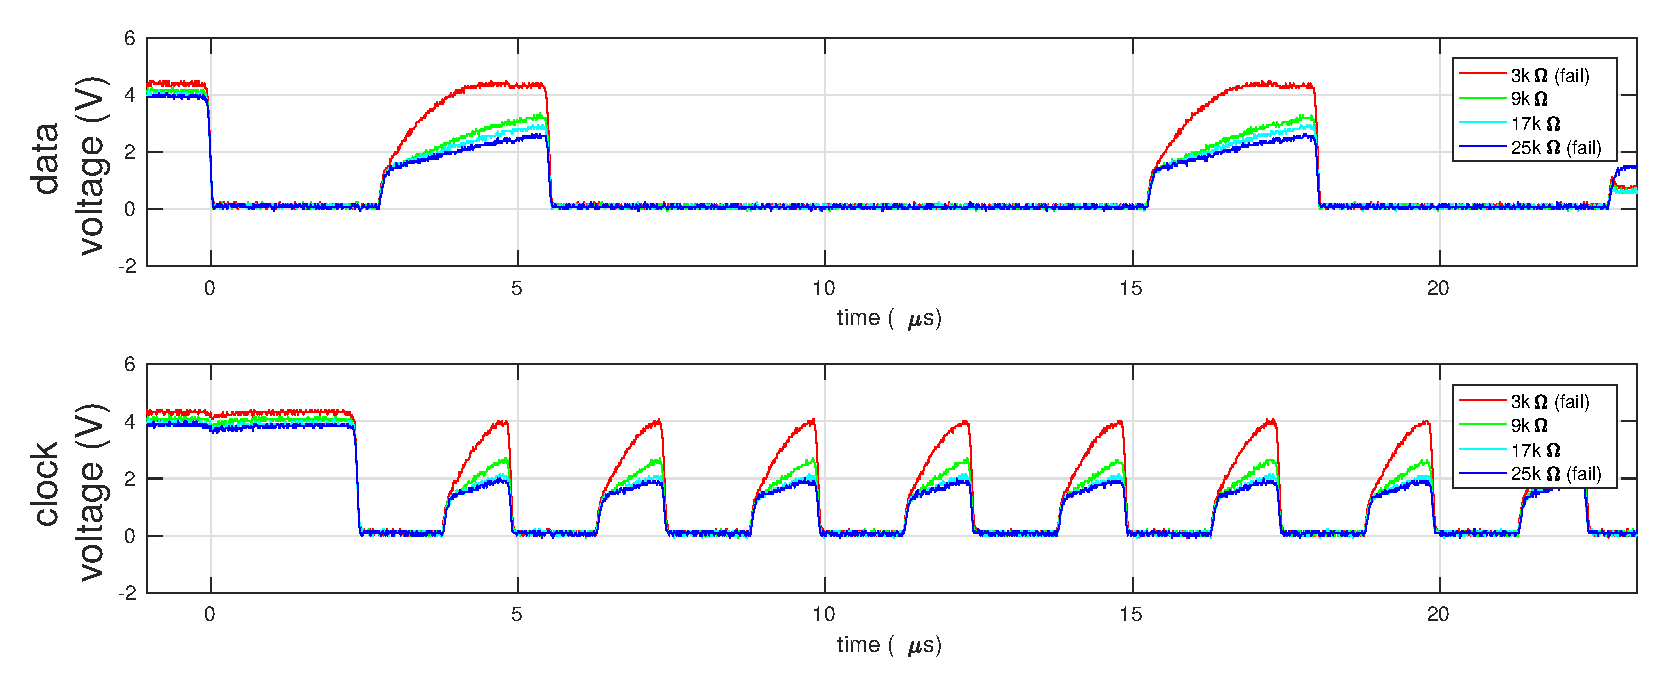
\includegraphics[width=1.0\textwidth]{2pt5microsec/PX_cropped.eps}
\caption{I2C waveform when the PX4Flow is connected by itself.}
\label{fig:PX}
\end{figure}
Similar trends are apparent in these waveforms compared to those of the LIDAR-Lite. For example, large pull-up resistors lead to slower transitions from logic low to logic high. Also note that in the $3 k \Omega$ case, the circuit has failed, even though the clock and data lines still seem to get close to 0V at low voltage. It is most likely that this case failed because the low voltage was too high, but it cannot be distinguished by the naked eye. Unlike the LIDAR-Lite, the PX4Flow does have a maximum working resistance. For the $9 k \Omega$, $17 k \Omega$ and $25 k \Omega$ waveforms, the clock and data lines only reach about half of the high voltage before they are brought back down to 0V by the next clock cycle. However, the $9 k \Omega$ and $17 k \Omega$ waveforms are successful while the $25 k \Omega$ is not. These results suggest that a waveform which appears to be quality, as in the $3 k \Omega$ case, may not actually be successful. On the other hand, a waveform which does not appear to be quality, as in the $9 k \Omega$ and $17 k \Omega$ case, may be successful. Therefore, it may not be possible to judge the quality of an I2C communication based on the waveforms alone.

\subsection*{Effect of Clock Speed}

Success of I2C communications depend on the I2C clock speed. A configuration which does not work at a fast clock speed may work if the speed is decreased. This is because the waveform will have more time to rise from low voltage. The disadvantage of reducing the clock speed is that communication is slower. An example is shown for the PX4Flow in Fig. \ref{fig:clockSpeedShift}.
\begin{figure}[ht]
\centering
%\includegraphics[width=1.0\textwidth]{photos/tester2.pdf}
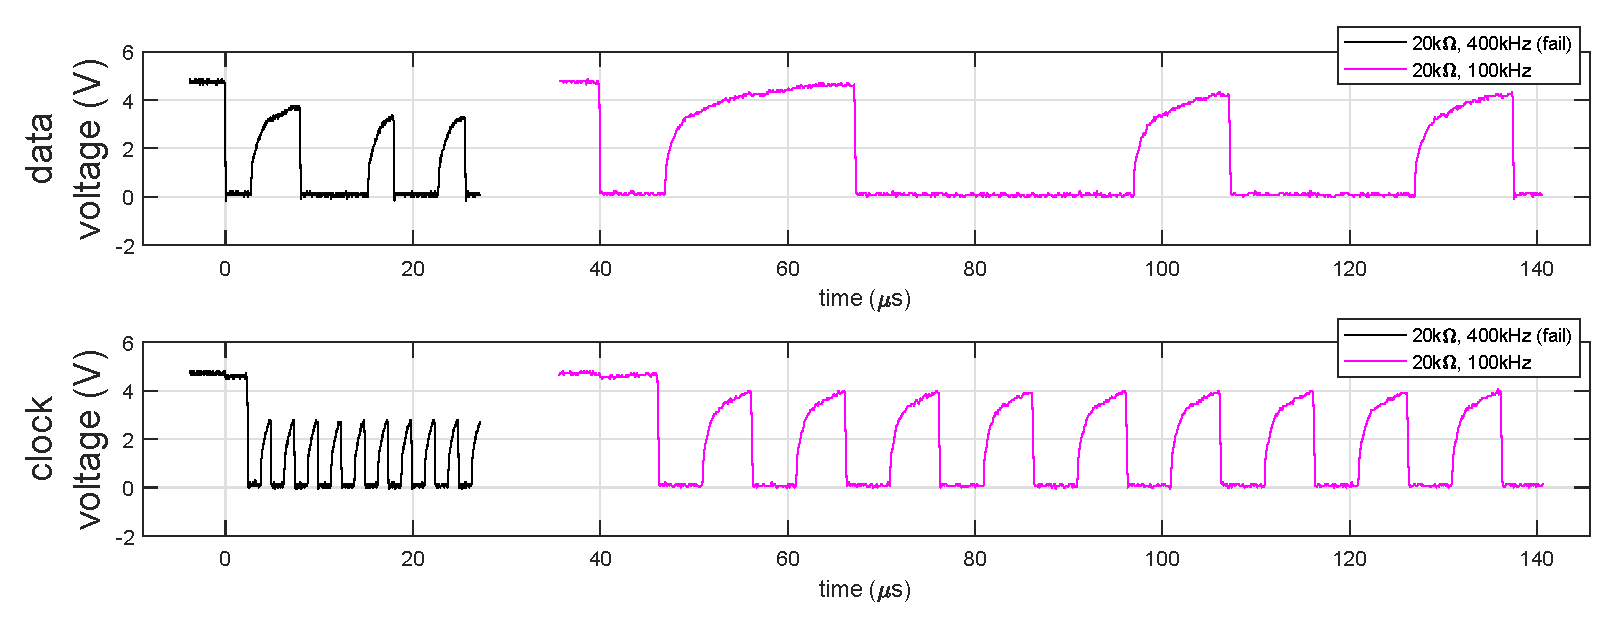
\includegraphics[width=1.0\textwidth]{5microsec/clock_shift_cropped.eps}
\caption{When the PX4Flow is connected by itself, $20 k \Omega$ pull-up resistors prevent the clock and data lines from nearing high voltage. However, if the clock speed is reduced, the lines have more time to rise, and the circuit works.}
\label{fig:clockSpeedShift}
\end{figure}
Since the pull-up resistors are the same in Fig. \ref{fig:clockSpeedShift}, the waveforms follow the same curve as they rise from low voltage. To see this, we can superimpose the clock and data curves, which is show in Fig. \ref{fig:clockSpeedCompare}.
\begin{figure}[ht]
\centering
%\includegraphics[width=1.0\textwidth]{photos/tester2.pdf}
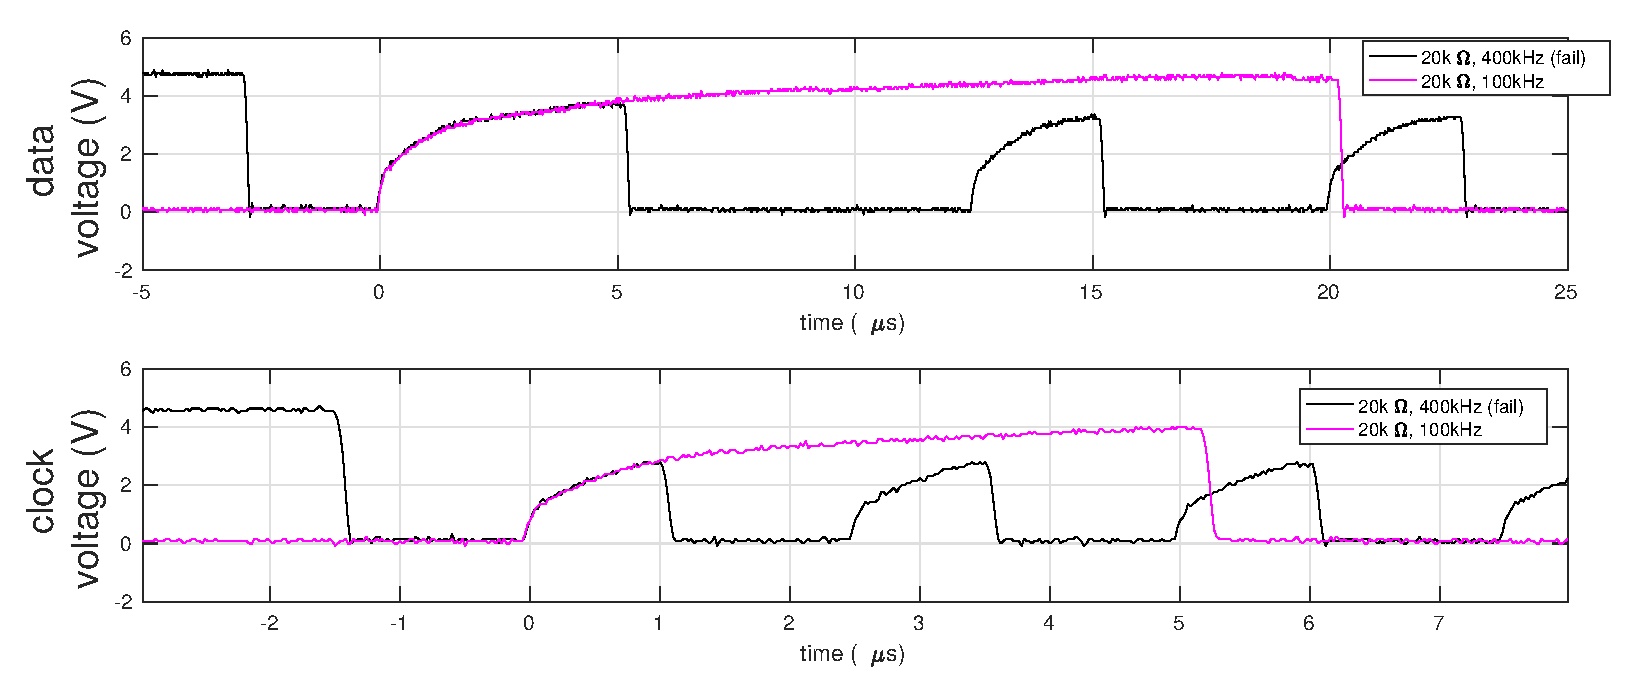
\includegraphics[width=1.0\textwidth]{5microsec/clock_compare_zoom_cropped.eps}
\caption{The same waveform as Fig. \ref{fig:clockSpeedShift}, but with the clock and data lines shifted to show that the waveforms rise from low voltage along the same curve.}
\label{fig:clockSpeedCompare}
\end{figure}

\section*{Conclusion}

We have described the process of connecting two sensors over I2C to a computer running embedded Linux. Since the sensors operate at different logic voltage levels than the computer, a converter circuit is required. Due to certain characteristics of the computer and sensors (e.g. whether there are internal pull-ups on any of the devices), it may be unclear which size pull-up resistors are needed for the circuit. So, it is helpful to first build the circuit with variable resistors so that appropriate values can be determined.


\section*{Appendix}

The C codes we used to communicate with the LIDAR-Lite and PX4Flow (named LL.c and PX.c) are located in the same directory as this PDF.


%https://wiki.gumstix.com/index.php/Category:How_to_-_i2c

\iffalse
\subsection*{C Code to communicate with the LIDAR-Lite, version 1}
%\tiny
\lstset{basicstyle=\tiny\ttfamily, language=C, commentstyle=\color{red}}
\lstinputlisting{LL.c}

\newpage

\subsection*{C Code to communicate with the PX4Flow (compiling this code requires linking the \texttt{ncurses} library)}
\lstset{basicstyle=\tiny\ttfamily, language=C, commentstyle=\color{red}}
\lstinputlisting{PX.c}
\fi

\end{document}
